\documentclass[aspectratio=169]{beamer}
\usepackage{cmap}
\usepackage{xfrac}
\usepackage[utf8]{inputenc}
\usepackage[T2A]{fontenc}
\usepackage[russian]{babel}
\usepackage{graphicx}
\graphicspath{ {./images/} }

\usetheme{Berkeley}

\title[Стохасти- ческая задача формирования теста]{Стохастическая постановка задачи формирования теста заданного уровня сложности с минимизацией квантили времени выполнения}
\author[Королев Егор \and Туманов Георгий]{Е.В.Королев \and Г.А.Туманов}
\institute[НИУ МАИ]{Московский авиационный институт (НИУ)}

\newcommand{\norm}[1]{\left\lVert#1\right\rVert}

\begin{document}
    \begin{frame}
        \maketitle
    \end{frame}

    \begin{frame}{План презентации}
        \tableofcontents
    \end{frame}

    \section{Введение}
    \begin{frame}{Введение}
        \begin{block}{LMS}
            С переходом на дистанционное образование активно развиваются системы управления обучением (LMS)\\
        \end{block}
    
        \begin{block}{Способ повышения качества дистанциооного образования}
            Применение анализа данных в LMS может повысить качество дистанционного образования\\
        \end{block}
    
        \begin{block}{За счет чего повышактся качество?}
            Сложность заданий оценивается экспертами, либо программно. Происходит адаптация контента под оцениваемый уровень знаний пользователя\\
        \end{block}
    \end{frame}

    \section{Постановка задачи}
    \begin{frame}{Логнормальная модель Ван дер Линдена}
        %\begin{block}{Логнормальная модель Ван дер Линдена}
            Пусть $Z=(z_1,\cdots,z_I)$ -- вектор заданий\\
            Ван дер Линден предположил, что логарифм времени $T_j^i$ (время ответа $j$-го пользователя на $i$-ю задачу) состоит из 3-х компонент:
            \begin{itemize}
                \item $\mu$ -- общая составляющая для всех пользователей и задач;
                \item $\beta_i$ -- индивидуальная сложность $i$-й задачи;
                \item $\tau_j$ -- особенности $j$-го пользователя, решающего задание.
            \end{itemize}
            Модель имеет вид:
            \begin{equation}
            \ln T_j^i = \mu + \beta_i + \tau_j + \varepsilon_{ij},
            \end{equation}
            где $\varepsilon_{ij} \thicksim \mathcal{N}(0,\sigma^2)$ -- независимые СВ
        %\end{block}
    \end{frame}


    \begin{frame}{Оценки параметров модели}
        %\begin{block}{Оценки параметров модели}
            Из ММП можно получить оценки модели:
            \begin{gather}
                \hat{\mu} = \dfrac{1}{I \cdot J} \sum\limits_{j=1}^J \sum\limits_{i=1}^I \ln t_j^i, ~~~  \hat{\beta_i} = \dfrac{1}{J} \sum\limits_{j=1}^J \ln t_j^i - \hat{\mu}, ~~~  \hat{\tau_j} = \dfrac{1}{I \cdot J} \sum\limits_{i=1}^I \ln t_j^i - \hat{\mu},\\
                \hat{\sigma^2} = \dfrac{1}{I \cdot J} \sum\limits_{j=1}^J \sum\limits_{i=1}^I \left( \ln t_j^i - \hat{\mu} - \hat{\beta_i} - \hat{\tau_j} \right)^2
            \end{gather}
        %\end{block}
    \end{frame}


    \begin{frame}{Плотность вероятности логнормального распределения}
        %\begin{block}{Плотность вероятности логнормального распределения}
            Таким образом, из модели (1) и с учетом оценок (2), (3) в качестве модели времени ответа пользователя на задание можно выбрать модель логнормального распределения с плотностью вероятности:
            \begin{equation}
                f(x,\tau_j,\beta_i,\sigma) = \dfrac{1}{x\sigma \sqrt{2\pi}}\exp \left\{ -\dfrac{1}{2} \left[ \dfrac{\ln x - (\hat{\mu} + \hat{\beta_i} + \hat{\tau_j})}{\hat{\sigma}} \right]^2 \right\}  
            \end{equation}
        %\end{block}
    \end{frame}


    \begin{frame}{Обозначения}
        \begin{block}{Матрица принадлежности}
            Разобъем множество заданий на $M$ различных типов, $I_m$ -- число заданий $m$-го типа.\\
            Пусть $A = \norm{ a_i^m }_{i=\overline{1,I}}^{m=\overline{1,M}},~~a_i^m =
                \begin{cases}
                    1, &z_i \in Z_m,\\
                    0, &z_i \notin Z_m.
                \end{cases}$
        \end{block}
    
        \begin{block}{Тестовый набор}
            Определим вектор $u\in\mathbb{R}^I$.\\
            Пусть $u_i =
                \begin{cases}
                    1, &\text{если задача $i$ попала в тестовый набор,}\\
                    0, &\text{иначе.}
                \end{cases}$\\
            Тестовым набором считаются $k$ заданий, для которых $u_i=1$.
        \end{block}
    \end{frame}


    \begin{frame}{Обозначения}
        \begin{block}{Cложность заданий}
            Введем $w\in\mathbb{R}^I$, $i$-я координата -- сложность $i$-го задания.\\
            Пусть изначально задаётся суммарная сложность теста, обозначаемая через $c$, которая определяется на основе экспертной оценки.
        \end{block}
    
        \begin{block}{Некоторые обозначения}
            Пусть в тестировании участвуют $N$ пользователей.\\
            Пусть $T_n^i$ -- случайное время, потребовавшееся пользователю $n$ на решение задачи $i$.\\
            И пусть $ T = \norm{ T_n^i }_{n=\overline{1,N}}^{i=\overline{1,I}}$.
        \end{block}
    \end{frame}
    
    
    \begin{frame}{Задача квантильной оптимизации}
        \begin{block}{Функция квантили}
            Пусть $\varphi$ -- общее время выполнения теста, которое неизвестно.\\
            Тогда для того, чтобы за некоторое оптимальное время все тестируемые могли выполнить выданный вариант теста с заданной вероятностью $\alpha$, рассмотрим функцию квантили:
            функцию квантили:
            \begin{equation}
                \Phi_\alpha(u)\triangleq\min\left\{\varphi:P\left\{\max_{n=\overline{1,N}}T_n u\leq\varphi\right\}\geq\alpha\right\}
            \end{equation}
        \end{block}
    \end{frame}
    
    
    \begin{frame}{Задача квантильной оптимизации}
        \begin{block}{Постановка задачи}
            Требуется составить множество индивидуальных тестовых наборов из $k$ заданий, принадлежащих различным типам, учитывая, что $k \geq M$.\\
            При этом, возможно отклонение от $c$ на какое-либо малое число $\varepsilon$ в большую, либо меньшую сторону.
        \end{block}
    \end{frame}

    \begin{frame}{Задача квантильной оптимизации}
        $$u_\alpha = Arg\min_{u\in\{0, 1\}^I}\left(\frac{\gamma\left|c-w^T u\right|}{\varepsilon} + \frac{(1-\gamma)\Phi_\alpha(u)}{2700}\right)$$
        $$\varphi_\alpha = \min_{u\in\{0, 1\}^I}\left(\frac{\gamma\left|c-w^T u\right|}{\varepsilon} + \frac{(1-\gamma)\Phi_\alpha(u)}{2700}\right)$$
        $$c-w^T u\leq\varepsilon$$
        $$w^T u-c\leq\varepsilon$$
        $$A^T u\geq e_M$$
        $$e_I^T u=k$$
    \end{frame}
    
    \begin{frame}{Дискретный аналог}
        Заменим непрерывные случайные величины $T_n^i$ на дискретные $\Theta_n^i$ со следующими распределениями:\\
        
        \begin{table}[]
            \begin{tabular}{|l||l|l|l|l|}
                \hline
                $\Theta_n^i$ & $\theta_n^i(1)$ & $\theta_n^i(2)$ & ... & $\theta_n^i(L_{ni})$\\ \hline
                $p_n^i$ & $p_n^i(1)$ & $p_n^i(2)$ & ... & $p_n^i(L_{ni})$\\ \hline
            \end{tabular}
        \end{table}
        
        где:\newline
        $0 = t_0 < t_1 < t_2 < ... < t_{L_{ni}-1} < t_{L_{ni}} = +\infty$ -- разбиение временного интервала\newline
        
        $\theta_n^i(\lambda)$ -- середины интервалов $[t_{\lambda-1}, t_\lambda], l=2,...,L_{ni}-1$\newline
        
        $\theta_n^i(1)$ и $\theta_n^i(L_{ni})$ -- квантили $T_n^i$ уровней 0.01 и 0.99 соответственно\newline
        
        $p_n^i(\lambda)=\int_{t_{\lambda-1}}^{t_\lambda}f(t, \tau_n, \beta_i, \sigma)dt$
    \end{frame}
    
    \begin{frame}{Функция квантили}
        Вместо матрицы $T$ будем использовать мктрицу $\Theta=||\Theta_n^i||$.
        
        Обозначим $\Theta_n$ -- n-ая строка матрицы $\Theta$. Тогда функция квантили примет вид:
        
        $$\Phi_\alpha(u)\triangleq\min\left\{\varphi:P\left\{\max_{n=\overline{1,N}}\Theta_n u\leq\varphi\right\}\geq\alpha\right\}$$
    \end{frame}
    
    \begin{frame}{Сведение к детерминированной задаче}
        Введём следующие обозначения:
        
        $$D=\prod_{n=1}^N\prod_{i=1}^I L_{ni}$$
        
        $\theta_d, d=1,...,D$ -- реализации случайной матрицы $\Theta$
        
        $$p=(p_1,...,p_D), p_d = P(\Theta=\theta_d)=\prod_{n=1}^N\prod_{i=1}^I P(\Theta_n^i=(\theta_d)_n^i)$$
        
        $$\overline{\varphi}=(\varphi,...,\varphi)^T\in R^N$$
        
        $\delta=(\delta_1,...,\delta_D)\in\{0,1\}^D$ -- вектор булевых переменных, определяющий доверительное множество
    \end{frame}
    
    \begin{frame}{Детерминированная задача}
        $$u^* = Arg\min_{u\in\{0, 1\}^I, \delta\in\{0, 1\}^D, \varphi\geq 0}\left(\frac{\gamma\left|c-w^T u\right|}{\varepsilon} + \frac{(1-\gamma)\varphi}{2700}\right)$$
        $$\theta_d u - \overline{\varphi}\leq(\theta_d e_I)\delta_d$$
        $$c-w^T u\leq\varepsilon$$
        $$w^T u-c\leq\varepsilon$$
        $$A^T u\geq e_M$$
        $$e_I^T u=k$$
        $$p\delta^T \leq 1-\alpha$$
    \end{frame}


    \section{Численный эксперимент}
    \begin{frame}{Численный эксперимент}
        Сформулируем задачу для одного студента на основе данных, полученных при обработке статистической информации системы дистанционного обучения МАИ CLASS.NET.
        
        $$N=1, D=\prod_{i=1}^I L_{1i}$$
        
        $M=3$ -- число типов заданий
        
        $I_m=10$ -- число различных заданий типа $m$, $m=1,2,...,M$
        
        $z_i^m$ -- $i$-е задание типа $m$, $m=1,2,...,M, i=1,2,...,I_m$
    \end{frame}

    \begin{frame}{Сложности заданий}
        Сложности $w_i^m$ заданий $z_i^m$ приведены в таблице:
        
        \begin{table}[]
\begin{tabular}{|l|l|l|l|l|l|l|l|l|l|l|}
\hline
$\sfrac{m}{i}$ & 1     & 2     & 3     & 4     & 5     & 6     & 7     & 8     & 9     & 10    \\ \hline
1   & 1.311 & 3.254 & 3.254 & 3.254 & 4.874 & 5.368 & 7.011 & 7.217 & 8.244 & 9.636 \\ \hline
2   & 4.132 & 6.902 & 2.121 & 3.436 & 2.456 & 5.359 & 6.902 & 7.283 & 7.815 & 9.399 \\ \hline
3   & 2     & 2.418 & 2.666 & 3.653 & 5.242 & 5.547 & 6.453 & 7.194 & 8.795 & 3.657 \\ \hline
\end{tabular}
\end{table}

	Потребуем суммарную сложность $c=29.46$ для теста из $k=5$ заданий.\newline $\varepsilon$ будем варьировать от 0.0004 до 0.004 с шагом 0.0001.
	
    \end{frame}
    
    \begin{frame}{Параметры распределений}
        Время $T_1^{im}$ на выполнение задания $z_i^m$ имеет логнормальное распределение $LN(\hat{\mu}+\hat{\beta}_i^m+\hat{\tau}_1, 0.31)$. Математические ожидания приведены в таблице:
    
    \begin{table}[]
\begin{tabular}{|c|c|c|c|c|c|}
\hline
$z_i^1$ & $\hat{\mu}+\hat{\beta}_i^1+\hat{\tau}_1$ & $z_i^2$ & $\hat{\mu}+\hat{\beta}_i^2+\hat{\tau}_1$ & $z_i^3$ & $\hat{\mu}+\hat{\beta}_i^3+\hat{\tau}_1$ \\ \hline
$z_1^1$ & 3.51 & $z_1^2$ & 4.72 & $z_1^3$ & 3.65 \\ \hline
$z_2^1$ & 3.92 & $z_2^2$ & 5.87 & $z_2^3$ & 3.73 \\ \hline
$z_3^1$ & 3.89 & $z_3^2$ & 3.83 & $z_3^3$ & 3.87 \\ \hline
$z_4^1$ & 3.91 & $z_4^2$ & 3.91 & $z_4^3$ & 3.96 \\ \hline
$z_5^1$ & 4.22 & $z_5^2$ & 3.87 & $z_5^3$ & 4.84 \\ \hline
$z_6^1$ & 4.63 & $z_6^2$ & 5.13 & $z_6^3$ & 4.95 \\ \hline
$z_7^1$ & 5.67 & $z_7^2$ & 5.25 & $z_7^3$ & 5.53 \\ \hline
$z_8^1$ & 5.71 & $z_8^2$ & 5.71 & $z_8^3$ & 5.89 \\ \hline
$z_9^1$ & 6.13 & $z_9^2$ & 5.94 & $z_9^3$ & 6.18 \\ \hline
$z_{10}^1$ & 6.39 & $z_{10}^2$ & 6.27 & $z_{10}^3$ & 3.88 \\ \hline
\end{tabular}
\end{table}
    \end{frame}
    
    \begin{frame}{Результаты эксперимента}
        Решим задачу на уровне доверия $\alpha=0.95$ при $\gamma=0$ и $\gamma=0.5$.\newline
        
        Обозначим $n_{det}$ -- количество решений, удовлетворяющих детерминированным ограничениям, $u^*$ -- оптимальный набор заданий, а $\psi^*$ -- оптимальное время в академических часах.
       	
       	\begin{table}[]
\begin{tabular}{|c|c|c|c|c|c|}
\hline
$\varepsilon$ & $n_{det}$ & $u^*,\gamma=0.5$ & $\psi^*,\gamma=0.5$ & $u^*,\gamma=0$ & $\psi^*,\gamma=0$ \\ \hline
0.0007 & 3 & $z_5^1,z_8^1,z_3^2,z_7^3,z_9^3$ & 0.5050 & $z_5^1,z_8^1,z_3^2,z_7^3,z_9^3$ & 0.5815 \\ \hline
0.0009 & 4 & $z_5^1,z_8^1,z_3^2,z_7^3,z_9^3$ & 0.4574 & $z_6^1,z_1^2,z_7^2,z_9^2,z_5^3$ & 0.5023 \\ \hline
0.003 & 21 & $z_5^1,z_8^1,z_3^2,z_7^3,z_9^3$ & 0.3408 & $z_6^1,z_8^1,z_1^2,z_6^3,z_8^3$ & 0.4710 \\ \hline
0.004 & 35 & $z_5^1,z_8^1,z_3^2,z_7^3,z_9^3$ & 0.3283 & $z_6^1,z_8^1,z_1^2,z_6^3,z_8^3$ & 0.4710 \\ \hline
\end{tabular}
\end{table}
    \end{frame}
    
    \begin{frame}{Анализ зависимости}
        Построим график зависимости оптимального решения $\psi^*$ от значения $\gamma$ при $\varepsilon=0.004$:
        
        \begin{center}
        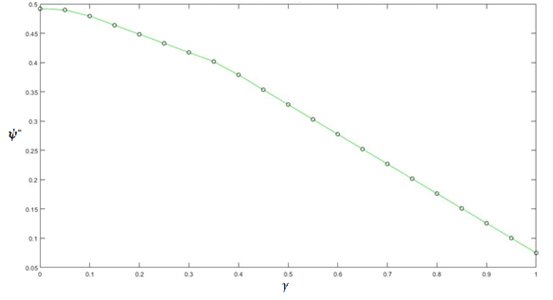
\includegraphics[scale=0.6]{plot}
        \end{center}
    \end{frame}
    
    \begin{frame}{Анализ результатов}
        При $\gamma\geq 0.5$ оптимальный набор не изменяется с увеличением $\varepsilon$ и является набором с наименьшим отклонением по сложности от $c$.\newline
        
        При $0\geq\gamma<0.5$ оптимальный набор меняется несколько раз при изменении $\varepsilon$.\newline
        
        Поэтому рассмотрим подробнее задачу при $\gamma=0$:
        
        \begin{table}[]
\begin{tabular}{|c|c|c|c|c|}
\hline
$\varepsilon$ & $u^*$ & $\varphi^*$(сек) & $\varphi^*$(мин) & $\psi^*$ \\ \hline
0.0004 & $z_5^1,z_8^1,z_3^2,z_7^3,z_9^3$ & 1570.0833 & 26.1681 & 0.5815 \\ \hline
0.0008 & $z_5^1,z_8^2,z_7^3,z_8^3,z_{10}^3$ & 1377.6667 & 22.9611 & 0.5102 \\ \hline
0.001 & $z_6^1,z_1^2,z_7^2,z_9^2,z_5^3$ & 1356.2    & 22.6033 & 0.5023 \\ \hline
0.002 & $z_6^1,z_7^1,z_4^2,z_7^3,z_8^3$ & 1328.025  & 22.1337 & 0.4919 \\ \hline
0.003 & $z_6^1,z_8^1,z_1^2,z_6^3,z_8^3$ & 1271.775  & 21.1963 & 0.4710 \\ \hline
\end{tabular}
\end{table}
    \end{frame}
    
    \begin{frame}{Время выполнения алгоритма}
        Зависимость затраченного времени выполнения алгоритма $t$ от значений $\varepsilon$:
        \begin{table}[]
\begin{tabular}{|c|c|} \hline
$\varepsilon$ & $t$(сек) \\ \hline
0.0004 & 4.189767  \\ \hline
0.0005 & 4.648206  \\ \hline
0.0006 & 4.521878  \\ \hline
0.0007 & 4.178228  \\ \hline
0.0008 & 5.498839  \\ \hline
0.0009 & 7.365371  \\ \hline
0.001  & 8.716812  \\ \hline
0.002  & 23.158336 \\ \hline
0.003  & 34.178394 \\ \hline
0.004  & 39.744152 \\ \hline
\end{tabular}
\end{table}
    \end{frame}
    
    \section{Заключение}
    \begin{frame}{Заключение}
        Была исследована математическая модель времени ответа пользователя и решена задача формирования ограниченных по времени тестов с заданной суммарной сложностью задания как одноэтапная задача квантильной оптимизации.

За основу модели времени ответа пользователя была взята модель ван дер Линдена. Непрерывные случайные величины были дискретизированы, и затем полученная задача была сведена к задаче математического программирования большой размерности.

В результате решения задачи с приведенными значениями параметров было получено 35 наборов тестовых заданий для $\varepsilon$=0.004. Полученные результаты численного эксперимента подтверждают адекватность предложенной модели. В итоге был разработан гибкий и удобный инструмент, который позволит формировать наборы тестовых заданий с учётом целей тестирования.

    \end{frame}
    
    \begin{frame}{Список литературы}
        \begin{itemize}
  			\item А. В. Наумов, Г. А. Мхитарян, Е. Е. Черыгова "Стохастическая постановка задачи формирования теста заданного уровня сложности c минимизацией квантили времени выполнения"
  			\item А. В. Наумов "Методы и алгоритмы решения задач стохастического линейного программирования с квантильным критерием"
		\end{itemize}
    \end{frame}

    \begin{frame}
        \centering
        \huge
        Спасибо за внимание!\\
    \end{frame}
\end{document}